% ------------------------------ MAPS ------------------------------ 
\begin{frame}\frametitle{Google Maps}

\begin{figure}[tc]
  \centering
  
\includegraphics[height=0.45\textheight,keepaspectratio=true]{images/maps_icon}
\end{figure}

Istnieje pewien ''problem'' z Google Maps oraz niektórymi innymi API. \\
\textbf{Nie są one dostępne bez odpowiedniego klucza oraz podpisania swojej aplikacji!}
\end{frame}


\begin{frame}\frametitle{MapsAPI key sign-up}
\begin{center}
  Rejestrujemy są po klucz na: \\
  http://code.google.com/intl/pl-PL/android/maps-api-signup.html \\
  BitLy: \textbf{http://bit.ly/mapsapiandroid}
\end{center}
\end{frame}


\begin{frame}[fragile]\frametitle{Zdobywanie MD5 klucza 'debug'}
\begin{lstlisting}
 keytool -list -alias androiddebugkey \
-keystore <path_to_debug_keystore>.keystore \
-storepass android -keypass android
\end{lstlisting}
\end{frame}


\begin{frame}[fragile]\frametitle{Zdobywanie Md5 klucza 'release'}

\textbf{keytool -list -keystore ~/android.keystore }

\begin{lstlisting}
Keystore type: JKS
Keystore provider: SUN

Your keystore contains 1 entry
android-key, Jul 3, 2011, PrivateKeyEntry, 
Certificate fingerprint (MD5): AA:AA:AA:AA...
\end{lstlisting}

\end{frame}


\begin{frame}\frametitle{Oto co dostaniemy:}
\begin{figure}
 \centering
 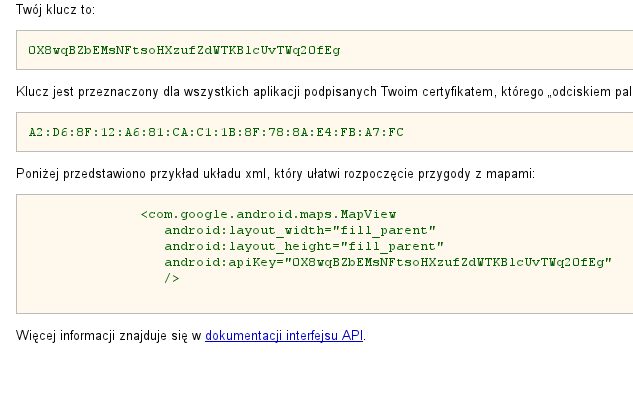
\includegraphics[width=\textwidth,keepaspectratio=true]{images/maps_get_key}
\end{figure} 
\end{frame}


\begin{frame}[fragile]\frametitle{Permissions}

W tym przypadku interesują następujące \verb|<uses-permission/>|:

\begin{itemize}
 \item \verb|android.permission.ACCESS_COARSE_LOCATION|
 \item \verb|android.permission.ACCESS_FINE_LOCATION|
\end{itemize}

oraz (skoro chcemy wyświetlić mapkę)
\begin{itemize}
 \item \verb|android.permission.INTERNET|
\end{itemize}

\pause
Dodatkowo jeszcze deklarujemy wykorzystanie biblioteki maps:
\begin{verbatim}
 <uses-library android:name="com.google.android.maps" />
\end{verbatim}

\textbf{Uwaga!}
\begin{lstlisting}
<application>
  <uses-library/> 
</application>
<uses-permission/>
\end{lstlisting}
\end{frame}

\begin{frame}\frametitle{Co na pewno się przyda?}
\begin{itemize}
 \item \textbf{LocationManager}
 \item \textbf{MapView}
 \item bardzo wygodny jest \textbf{MapActivity}
 \item tip: dostępny jest \textbf{GPS} i \textbf{NETWORK} location provider
\end{itemize}
\end{frame}
 
\begin{frame}[fragile]\frametitle{Zadanie: Google Maps App}
\begin{itemize}
 \item mapka, wycentrowana na obecnym położeniu telefonu
 \item podczas odświeżenia lokalizacji ma pojawiać się Toast z nową lokalizacją (oraz recentrujemy mapkę)
 \item obecne położenie ma być zaznaczone markerem: \textbf{http://bit.ly/gmapmark}
 \item dodatkowe: w przypadku oddalenia się od miejsca X (dowolne) należy odpalić '\textbf{alarm}'
 \item dodatkowe: zaskocz nas czymś!
\end{itemize}
\end{frame}
